\section{COSH Hyperbolic Cosine Function}

\subsection{Usage}

Computes the hyperbolic cosine of the argument.
The syntax for its use is
\begin{verbatim}
   y = cosh(x)
\end{verbatim}
\subsection{Function Internals}

The \verb|cosh| function is computed from the formula
\[
   \cosh(x) = \frac{e^x+e^{-x}}{2}
\]
For \verb|x| complex, it follows that
\[
   \cosh(a+i*b) = \frac{e^a(\cos(b)+i*\sin(b)) + e^{-a}(\cos(-b)+i*\sin(-b))}{2}
\]
\subsection{Examples}

Here is a simple plot of the hyperbolic cosine function
@>


\centerline{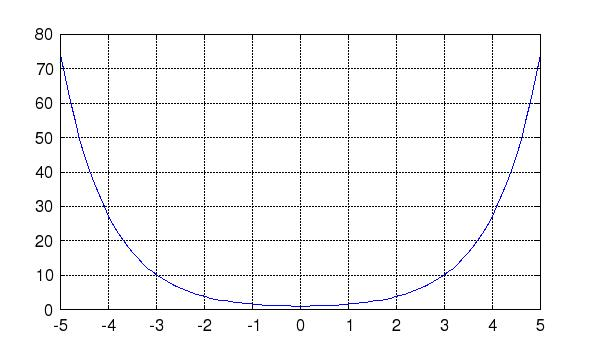
\includegraphics[width=8cm]{coshplot}}

